\chapter{Programs and Control}
\label{ch:programs-control}

Write two instructions on adjacent lines. Why should the second run after the
first? Position on the page is an assembly convention. The machine follows its
program counter. An ordinary instruction advances that counter. A branch may
replace the ordinary next address. A trap or halt permits no next step at all.

Control turns a list of instructions into a path through states. That path,
not the layout of the listing, is the execution we will reason about.

\begin{keyidea}[title={A program listing is not an execution}]
A listing arranges instructions for a reader. An execution follows program
counter values through complete states. Sequential layout matters only because
the instruction semantics assigns it an address rule.
\end{keyidea}

\section{A program supplies the bytes}

\begin{definition}[title={A0 program}]
An A0 \keyterm{program} is a finite immutable map of instruction bytes,
together with an entry program counter and a declared code-address range.
Every A0 instruction occupies four bytes and begins at an address divisible
by four.
\end{definition}

Object \obj{A0.def.program} records this object. The data memory in machine
state and the program's code map are separate. The first A0 model cannot
change its own instructions by storing to data memory.

The program counter selects four bytes from the code map. A normal
non-control instruction advances \(pc\) by four modulo \(2^w\). A fetch traps
if \(pc\) is not divisible by four or if the four-byte range is incomplete.
The fact that another instruction happens to be printed below the current one
does not repair either failure.

The code range also prevents a valid four-byte pattern from becoming an
instruction merely because the bytes exist somewhere. A fetch must begin at a
declared code address, satisfy the four-byte alignment rule, and find all four
bytes. Decoding begins only after those conditions hold.

For now, a hand trace will show both bytes and decoded instructions. Chapter 6
will explain how the decoder obtains the instruction instance and why illegal
encodings are part of program behavior.

\subsection{Stored programs made control a data-dependent process}

Before stored programs, changing a machine's task could mean rewiring,
reconfiguring switches, or replacing an external sequence of control media.
Placing instructions in addressable storage made the next operation depend on
a small part of machine state: the program counter. Conditional transfer then
made that counter depend on values produced during the calculation.

The historical gain was not merely convenience. A finite body of code could
repeat, select among cases, and call reusable routines. The same bytes could
process inputs of many sizes because the path and number of visits were chosen
while the program ran. A short program became a description of a potentially
long computation.

That foundation remains visible today beneath compilers, operating systems,
interpreters, and virtual machines. Optimizers rearrange control while trying
to preserve observed behavior. Security mechanisms restrict indirect targets.
Debuggers reconstruct paths from partial evidence. Formal verification asks
whether every path from an allowed entry respects a contract. Each task begins
with the same modest question: which successor states does the program admit?

\begin{archive}[title={A finite description can govern unbounded time}]
A program map is finite, but execution may revisit its addresses without a
fixed limit. The mystery is not an infinite program hidden in memory. It is
iteration: a finite transition rule applied again to each new state.
\end{archive}

\section{A trace through states}

\begin{definition}[title={A0 execution trace}]
An A0 \keyterm{execution trace} is a finite sequence
\[
  S_0,S_1,\ldots,S_k
\]
in which each adjacent pair is linked by one A0 step. A bounded runner reports
whether the last state halted, trapped, exhausted the step bound, or remains
able to continue.
\end{definition}

\begin{figure}[htbp]
\centering
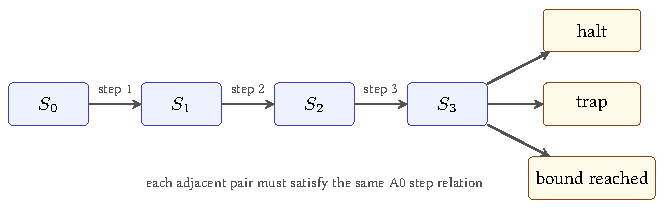
\includegraphics[width=0.94\textwidth]{figures/a0-trace}
\caption{A bounded trace is a sequence of checked adjacent steps. Reaching a
bound is distinct from reaching a terminal machine outcome.}
\figalt{States S0 through S3 connect by steps, then lead separately to halt, trap, or a reached bound.}
\label{fig:a0-trace}
\end{figure}

The diagram's three exits do not mean that one state has three outcomes. A
particular run produces one result. The fan-out records the cases the runner
must distinguish. If the last state is running when the requested bound is
used up, the runner reports that fact without changing the machine outcome to
halted or trapped.

Object \obj{A0.def.trace} records this relation. A trace contains its initial
state. A three-instruction execution that finishes normally therefore contains
four states: the state before the first step and one state after each step.

Consider this width-eight decoded program, with instructions at addresses
0, 4, 8, and 12:

\begin{codelisting}[language={},caption={A short A0 program}]
movi r1, 5
movi r2, 3
add  r0, r1, r2
halt
\end{codelisting}

Begin with \(pc=0\), a running outcome, and arbitrary old values in the three
registers. The first step writes 5 to \(r_1\) and sets \(pc=4\). The second
writes 3 to \(r_2\) and sets \(pc=8\). The third writes 8 to \(r_0\), sets
\(Z=0,N=0,C=0,V=0\), and sets \(pc=12\). The fourth changes the outcome to
halted. It preserves the registers, memory, program counter, and conditions.
There is no fifth step.

\begin{example}[title={The complete four-instruction trace}]
The trace contains five states, not four. \(S_0\) is the input. \(S_1\) has
\(r_1=5\) and \(pc=4\). \(S_2\) also has \(r_2=3\) and \(pc=8\). \(S_3\)
also has \(r_0=8\), cleared conditions, and \(pc=12\). \(S_4\) changes only
the outcome to halted. Every omitted component is preserved at each named
step.
\end{example}

Writing the states rather than only the instruction outputs exposes two
common counting errors. The initial state belongs to the trace, and halt is an
executed transition rather than the absence of one. The statement ``four
instructions ran'' therefore corresponds to four edges and five vertices.

This trace is straight-line because every non-halt step uses its ordinary next
address. The definition still comes from the program counter. That distinction
will let a branch choose another path without changing what a trace is.

\subsection{Multi-step execution is the closure of one-step execution}

The instruction semantics defines one edge \(S\to S'\). Program theorems
usually concern zero or more edges. Write
\(S\mathrel{\to^{k}}T\) when there is a trace of exactly \(k\) steps from
\(S\) to \(T\). The zero-step case relates every state to itself. The
successor case composes one step with a \(k\)-step execution.

\begin{figure}[htbp]
\centering
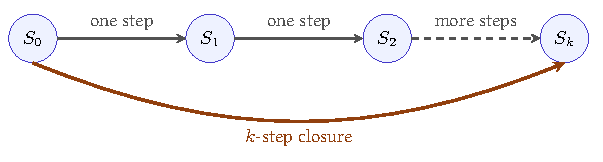
\includegraphics[width=0.82\textwidth]{figures/multi-step-closure}
\caption{Multi-step execution is built from checked adjacent one-step
transitions. It does not introduce another instruction semantics.}
\figalt{States S0, S1, S2, and Sk are joined by one-step arrows, with a curved arrow representing their k-step closure.}
\label{fig:multi-step-closure}
\end{figure}

This definition supplies a composition law. If
\(S\mathrel{\to^{m}}T\) and \(T\mathrel{\to^{n}}U\), concatenating the
traces gives \(S\mathrel{\to^{m+n}}U\). The shared state \(T\) appears
once in the combined state sequence even though it closes the first trace and
opens the second.

\begin{proofkit}[title={Concatenating execution traces}]
Take the state sequence from \(S\) to \(T\) and append the second sequence
after omitting its first copy of \(T\). Every adjacent pair comes from one
of the original traces, including the join because both use exactly the same
state \(T\). The edge count is \(m+n\), while the state count is
\(m+n+1\).
\end{proofkit}

Determinism gives uniqueness at a fixed step count. If each running state has
at most one successor, two \(k\)-step traces from the same initial state have
the same states at every position. That fact justifies speaking of \emph{the}
bounded A0 run after the program, initial state, and bound are fixed. It does
not guarantee that a successor exists: halt, trap, or invalid fetch can end the
trace earlier.

Prefix closure is equally important. Every initial segment of a valid trace is
a valid trace. A checker can therefore validate a long execution one adjacent
pair at a time. The converse requires matching endpoints: two separately
valid traces cannot be joined merely because their printed instruction
addresses look compatible.

\section{A branch asks state a question}

A0 separates comparison from conditional control. The instruction
\code{cmp r1, r2} computes the width-\(w\) subtraction \(R[r_1]-R[r_2]\) to
set \(Z,N,C,V\); it does not write the subtraction result
to a register. A later conditional branch reads selected condition bits.

Suppose \(r_1\) and \(r_2\) both contain 5. After \code{cmp r1,r2}, \(Z=1\).
The instruction \code{branch.eq 2} then takes its relative target:
\[
  pc+4+4\mathbin{\cdot}2.
\]
If the branch itself begins at address 4, the target is 16. If the two
registers differ, \(Z=0\), and the same branch advances to address 8.

\begin{figure}[htbp]
\centering
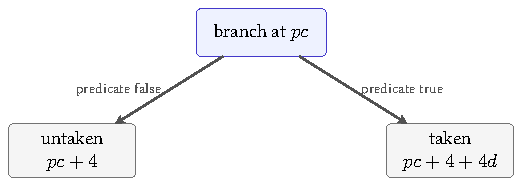
\includegraphics[width=0.72\textwidth]{figures/branch-fork}
\caption{An A0 conditional branch chooses between the sequential address and
a target measured from that sequential address.}
\figalt{A branch at pc goes to pc+4 when false and pc+4+4d when true.}
\label{fig:branch-fork}
\end{figure}

The offset is relative to the sequential address, not to the current address.
A faulty rule that uses \(pc+4\mathbin{\cdot}2\) lands at 12 in this example.
That near miss is useful: the wrong trace still reaches an aligned instruction,
so a test must check the target rule rather than merely alignment.

The displacement \(d\) is a signed eight-bit value before extension to the
word width. Multiplication by four scales instruction units to byte addresses.
Adding it to \(pc+4\) makes displacement zero name the next instruction, not
the branch itself. A backward branch uses a negative displacement. All three
steps—sign extension, scaling, and choice of base—belong to the target rule.

\begin{tryit}[title={Taken, untaken, and backward}]
Place a branch at address 20. Compute both successors for displacements 0, 2,
and -3. For each displacement, separate the sequential address from the taken
target before deciding which predicate value chooses it.
\end{tryit}

The paired architectures place the predicate differently. A later RV64
conditional branch will compare register values as part of the branch
instruction. A common selected x86-64 pattern will have one instruction set
condition flags and a later conditional jump read them. A0 deliberately uses
the second broad shape. The comparison dimension is where the branch predicate
lives, not which family receives the simpler label.

\subsection{Control-flow graphs summarize possible local edges}

A \keyterm{basic block} is a sequence entered at its first instruction and
left only at its end under the chosen graph construction. Ordinary
fallthrough keeps execution inside the block. A branch, jump, halt, trap, or
declared entry point creates a boundary. The exact partition depends on which
targets and failures the analysis includes.

A control-flow graph places these blocks or instruction addresses at nodes and
adds possible successor edges. For a direct conditional branch, the local
graph usually includes the fallthrough and taken target even if one predicate
is impossible under the program's input premise. A trace selects one of those
edges in one state. A state invariant can later remove an infeasible edge.

The distinctions prevent three common overclaims:

\begin{enumerate}
\item absence from sampled traces does not make a graph edge unreachable;
\item presence in a syntactic graph does not prove that an allowed state can
take the edge; and
\item local reachability of an address does not prove that fetching and
decoding there succeeds.
\end{enumerate}

Reachability begins at the declared entry state or entry set. Inductively, the
entry is reachable, and a successor of a reachable running state is reachable.
This definition is semantic because it mentions states and steps. Graph
reachability over a conservative edge set is an overapproximation unless every
edge has also been shown feasible.

\begin{definition}[title={Control point}]
A control point is an address or phase at which a proof states a relation or
invariant. It need not be every instruction boundary. Loop heads, procedure
entries, call returns, and final exits are common choices. The proof must still
justify the intervening steps between consecutive control points.
\end{definition}

Control points let two machines take different numbers of instructions while
supporting the same higher-level argument. They also keep loop invariants
readable: the invariant can describe the state at the head rather than every
temporary state inside the body.

\section{Four ways a bounded run can end}

A halted trace has executed \code{halt}. A trapped trace has encountered a
declared failure, such as an invalid fetch or memory range. Both have a final
state with no successor, but one records normal completion and the other
records failure.

A third run may consume its requested step bound while its last state is still
running. The runner has stopped looking; the program has not necessarily
stopped. This is \keyterm{bound exhaustion}. A fourth result can return a
running state before a larger calling procedure decides whether to take
another step. Neither result proves termination or looping.

The difference matters even for a one-instruction loop. Run an unconditional
branch back to itself for one hundred steps. The bounded trace contains one
hundred valid transitions and a running final state. It is evidence about that
prefix. To show that execution never halts requires an argument about every
later step, such as an invariant that the program counter always returns to the
same instruction and no state component can cause another path.

A finite state description can thus give rise to an unbounded question. The
machine is small; time need not be.

\begin{warning}[title={A bound is a resource limit, not a semantic verdict}]
Reaching 1,000 valid steps establishes a 1,000-step prefix. It does not show
that the program halts at step 1,001, runs forever, or eventually traps. Each
of those conclusions needs evidence beyond the exhausted run.
\end{warning}

A loop proof supplies that further evidence by identifying an invariant. For
the unconditional self-branch, the program counter returns to the same
address, the branch preserves every other state component, and the outcome
remains running. Applying the same rule again recreates the same state. An
induction over the number of steps then covers every finite prefix. The proof
uses the transition rule, not the patience of the runner.

\subsection{Invariants prove safety; variants can prove termination}

An invariant is a predicate intended to hold whenever execution reaches a
chosen control point. The proof has two obligations. Initialization shows that
the entry path establishes the predicate. Preservation assumes it at one
visit, executes the loop segment, and shows it again at the next visit. By
induction, the invariant holds at every reached visit.

The invariant need not describe all state. It should carry exactly the facts
needed for the next iteration and final theorem: counter bounds, address
validity, preserved memory, relationships among registers, or a condition
connecting machine words to mathematical values. A weak invariant may be true
but unable to prove safety. An unnecessarily strong one may fail because it
mentions scratch state that legitimately changes.

\begin{proofkit}[title={Loop-invariant induction}]
Let \(I(S)\) be the invariant at loop head \(h\). Prove that the entry
execution reaches a state \(S_0\) with \(pc=h\) and \(I(S_0)\). Next,
for an arbitrary reachable \(S\) with \(pc=h\) and \(I(S)\), prove that
one loop iteration either exits under the intended postcondition or reaches a
new head state \(S'\) satisfying \(I(S')\). Induction covers every finite
number of completed iterations.
\end{proofkit}

This establishes preservation properties but not necessarily termination. A
\keyterm{variant} adds a value in a well-founded order, commonly a natural
number, that strictly decreases on every returning iteration. If the body
cannot get stuck and the variant cannot decrease forever, execution must
eventually leave the loop.

Safety and termination can therefore split. An infinite self-branch has the
invariant that the complete state repeats, which proves it never reaches bad
state under the model. It has no decreasing natural variant and does not
terminate. A countdown loop can have both an invariant keeping its counter in
range and a variant equal to the remaining count.

The exit theorem uses the invariant plus the negated continuation condition.
For example, if an invariant states \(0\leq r\leq n\) and the loop continues
exactly while \(r>0\), reaching the ordinary exit yields \(r=0\). The
control predicate is part of the mathematical conclusion, not merely a jump
detail.

\subsection{Partial and total correctness answer different questions}

Suppose the four-instruction example has the postcondition \(r_0=8\). We can
ask two different questions. First: whenever the program reaches its normal
exit, does the final state satisfy that postcondition? Second: from every
allowed initial state, does the program actually reach that exit? The first
question concerns \keyterm{partial correctness}. The second question, joined
to the first, gives \keyterm{total correctness}.

For the straight-line example, the distinction is easy to miss. Fetch and
decode succeed at four consecutive addresses, each instruction has one
successor, and the fourth instruction halts. The same trace that establishes
the result also establishes arrival at the result. Loops separate the two
obligations. An invariant may say exactly what would be true at the exit while
providing no reason that the exit will ever be reached.

\begin{warning}[title={A true implication may say nothing about arrival}]
The implication \emph{if the program halts, then \(r_0=8\)} is true for a
program that never halts and never writes 8. Partial correctness is useful,
but it must not be read as a termination claim. To obtain total correctness,
add a termination argument under the same initial-state premise.
\end{warning}

Traps require another separation. A contract may permit them, rule them out,
or assign them their own postcondition. If normal exit and trap are both
terminal outcomes, a claim about halted states alone says nothing about
trapped states. A robust program theorem therefore partitions the possible
outcomes before stating what must hold in each part.

A bounded runner does not collapse this distinction. If the bound is reached,
the runner has established a finite prefix. A sufficiently large bound may
cover every run only when another argument supplies a uniform upper bound on
execution length. That bound is a theorem premise or conclusion external to
the step relation; it is not hidden inside the number entered at the command
line.

This vocabulary will matter when later chapters compare two programs. One may
produce the right value whenever it exits but diverge on an input where the
other program halts. Agreement on final register values then fails to capture
the difference in behavior.

\section{Replacement inside a context}

Suppose programs \(p\) and \(q\) leave the same value in \(r_0\) for every
allowed initial state. Can one replace the other before any suffix \(r\)?

No. Let \(p\) also leave \(r_3=0\), while \(q\) leaves \(r_3=1\). They agree
under an observation of \(r_0\). Choose a suffix that copies \(r_3\) into the
final output. The suffix exposes the difference that the earlier observation
discarded.

The same counterexample works with condition state. Two prefixes may agree on
registers while setting \(Z\) differently. A suffix beginning with
\code{branch.eq} can choose different paths. Agreement on an output before the
branch is not enough.

The repair is exact. Suppose \(p\) and \(q\), from every allowed initial
state, finish with the same outcome and agree on every state component that
the deterministic suffix can read. The first suffix instruction then receives
indistinguishable inputs. It produces matching values for the components
needed by the second instruction, and the same argument repeats through the
suffix. The final states agree under the declared observation.

The argument is a reader proof of a contextual rule, not yet a general theorem about
all programs. Its premises need a precise read set, termination account, and
observation. Later chapters will formalize those conditions as equivalence and
refinement. For now, the counterexample has done its job: local replacement
depends on context unless the state relation covers what the context can see.

\begin{proofkit}[title={\iconProofKit\ Replacement through a deterministic suffix}]
Let two prefixes finish in running states that agree on every component the
first suffix instruction can read. Determinism gives matching relevant outputs
after that instruction. Repeat the argument for each later suffix instruction.
If both executions reach the end under the same outcomes, their final states
agree under the declared observation. The proof fails when a suffix reads a
component on which the prefix states disagree.
\end{proofkit}

The premise must follow the path actually taken. A suffix containing a branch
may read one set of components on one path and another set on a second path.
Agreement sufficient to choose the same first branch can simplify the rest of
the proof. Agreement only at the final output of the prefixes cannot.

We can describe the required agreement with a projection \(\pi\). The
projection retains the components a context may observe: perhaps selected
registers and the outcome, or perhaps registers, conditions, reachable memory,
and program bytes. If \(\pi(S_p)=\pi(S_q)\) after the two prefixes, replacement
is sound only when every permitted context treats states with the same
projection alike. Choosing \(\pi\) is therefore part of the claim, not a
formatting choice made after the executions have been compared.

A context can observe more than its final arithmetic result. It can branch on
a condition, load from an address changed by the prefix, encounter a fault on
one path, or use an indirect target obtained from a register. In a machine
with writable code, it might even fetch different instruction bytes. A proof
that forgets any such input licenses a suffix designed to reveal the forgotten
difference.

\begin{sidebar}[title={Closed-program agreement can be weaker}]
Two complete programs may agree under a final-output observation even though
their intermediate states differ. That can be enough when nothing will be
appended and no external observer sees the intermediate states. Replacement
inside an arbitrary context is stronger: the context becomes an observer and
may turn a hidden difference into a visible one.
\end{sidebar}

The useful projection is rarely the whole physical machine. It is the state
named by the model and exposed to the admitted contexts. A0 excludes caches,
timing, interrupts, and self-modifying code, so an A0 contextual result cannot
settle whether two real implementations leak different timing information.
Conversely, retaining every A0 register when the suffix reads only one may be
safe but needlessly strict. Later equivalence proofs will balance these two
errors: forgetting an observable component and preserving irrelevant detail.

\begin{example}[title={A context exposes one forgotten bit}]
Prefix \(p\) and prefix \(q\) both leave \(r_0=7\), but they leave different
values of \(Z\). Append a suffix that branches to write 0 or 1 into \(r_0\)
according to \(Z\). The composed programs now disagree on their visible
output. The suffix did not create the earlier difference; it converted hidden
state into an observed register.
\end{example}

\section{The implementation boundary}

An Axeyum runner for A0 must fetch, decode, and step through the program while
keeping halt, trap, bound exhaustion, and continued execution distinct.
Object \obj{OP.a0.run} records that obligation.

The introductory Axeyum run should print a trace a person can compare with the
book. Each row needs the step number, program counter, decoded instruction,
changed components, and outcome. A replay command should consume the same
initial state and program bytes, not a second handwritten formula that merely
resembles them.

\begin{figure}[htbp]
\centering
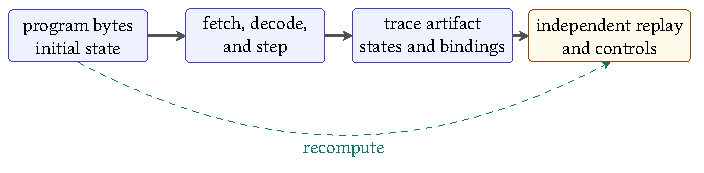
\includegraphics[width=0.9\textwidth]{figures/trace-artifact-replay}
\caption{A future Axeyum trace route binds program bytes and initial state to
an artifact, then independently replays every derived transition and control.}
\figalt{Program bytes and initial state enter fetch decode and step, produce a trace artifact, and pass to independent replay and controls that also recompute from the inputs.}
\label{fig:trace-artifact-replay}
\end{figure}

The artifact should not trust its own change summary. It stores complete states
or a lossless initial state plus checked deltas; the replayer reconstructs each
successor and compares every component in scope. It also decodes from the bound
program bytes at the recorded program counter. A printed mnemonic is a display
field, not semantic input.

Termination labels need independent derivation. The replayer inspects the last
machine outcome and the requested bound. Halt and trap must arise from actual
steps. Bound exhaustion requires a running final state and exactly the allowed
number of steps. A continued-execution result may expose a shorter prefix
without claiming that the machine stopped.

A solver-backed question comes later. It may ask whether two short A0 programs
can finish with different observations under an input premise. If the answer
is yes, the model must decode into an initial state and replay into two traces.
If the answer is no, the route needs the generated formula, scope, and
independent checking boundary. The trace printer remains useful in both cases
because it connects the verdict to executable steps.

The controls attack control itself. Mutate a relative target by four bytes.
Try to execute after a trapped state. Try to execute after halt. Report a
running state at a finite bound as if the program had terminated. Each error
can preserve the arithmetic destination for a while, which is why trace
checking must inspect more than the final register.

Add structural controls as the implementation grows. Remove one intermediate
state while leaving the endpoints. Duplicate a state without a matching step.
Change the program digest after producing the trace. Alter an unobserved
register in one successor. Each mutation attacks a different binding:
adjacency, step count, program identity, or full-state preservation.

For a first Python lesson, the public surface can stay small: construct an A0
program from bytes, construct a complete initial state, request a bounded run,
print the returned trace, and invoke verification. The Rust layer should own
fetch, decode, step, serialization, and checking. Python organizes the lesson
and renders the explanation; it must not supply an alternate transition rule.

This runner does not accompany the draft. The traces in this chapter are hand
executions of the stated A0 rules. They establish how the future runner must
behave on these examples; they do not claim that all A0 traces have already
been checked.

\section{One complete Part I trace}

We can now name every layer in the four-instruction example. The immediate
bytes denote width-eight words. Registers and conditions belong to complete
state. Each decoded instruction has explicit operands and effects. The
program counter selects immutable code bytes and advances by four. The add
uses modular arithmetic and records facts about the mathematical sum. The
\code{halt} outcome prevents another step. An observation may expose \(r_0\)
alone, but the trace itself retains the rest.

Nothing in that account depends on calling A0 a RISC or CISC machine. Those
labels would add less information than the rules we have printed. When the
book turns to real architectures, the same inventory will let us compare one
choice at a time.

One boundary remains even in our tiny example. We have written decoded
instructions beside the trace. A processor receives bytes. Before an
instruction can transform state, those bytes must select one legal operation,
operand form, and length---or cause a decoding failure. Part II begins at that
boundary.

\section{Exercises}

\begin{enumerate}
\item \textbf{Execute.} Run the four-instruction program in this chapter from
\(pc=0\), with every register initially zero. List every complete state
component that changes at each step.
\item \textbf{Break.} Replace the taken branch target rule
\(pc+4+4d\) with \(pc+4d\). For a branch at address 4 with displacement 2,
show the two traces diverging at their next program counters.
\item \textbf{Prove.} Give an invariant showing that an unconditional
zero-displacement branch returns to the same instruction under the A0 target
rule. Explain why any finite bounded run alone would be weaker.
\item \textbf{Transfer.} Write one register-predicate branch pattern for the
later RV64 slice and one compare-then-jump pattern for the later x86-64 slice.
List the state read by each branch instruction itself.
\item Construct two one-instruction prefixes that agree on \(r_0\) but differ
on a component read by a suffix. Give the suffix and trace both composed
programs.
\item Act as the runner for a program that traps on its second instruction.
Show why appending a valid third instruction creates no third transition.
\item State the exact result of running a still-running program at bounds 0,
1, and 2. Do not use the words halt or loop unless the trace warrants them.
\item \textbf{Execute.} For the program in this chapter, list the five states
as rows with \(pc\), changed registers, condition bits, and outcome. Confirm
that each adjacent pair satisfies exactly one step.
\item \textbf{Break.} Make a runner label bound exhaustion as halt. Give a
one-instruction self-loop on which the faulty label changes the observable
outcome.
\item \textbf{Prove.} Formalize the self-loop argument by induction on the
number of transitions. State the invariant and the base and induction cases.
\item \textbf{Transfer.} For one planned RV64 branch and one planned x86-64
conditional jump, list the state needed to select the path and the rule needed
to calculate both target addresses.
\end{enumerate}
